%% Shared: as_slave_bpi, used by every Wishbone peripheral (both variants)
%%%%%%%%%%%%%%%%%%%%%%%%%%%%%%%%%%%%%%%%%%%%%%%%%%%%%%%%%%%%%%%%%%%%%%%%%%%%%
\subsection{Wishbone Slave BPI (\texttt{as\_slave\_bpi})}
\label{subsec:asSlaveBpi}
%%%%%%%%%%%%%%%%%%%%%%%%%%%%%%%%%%%%%%%%%%%%%%%%%%%%%%%%%%%%%%%%%%%%%%%%%%%%%

\subsubsection{History}
\begin{table}[H]
\caption{History of as\_slave\_bpi}
\label{tab:asSlaveBpiHist}
\centering
\begin{tabularx}{\textwidth}{|l |l |l |X|}
  \hline
  Version & Date & Author & Change \\
  \hline
  \hline
  0.1 & 2026-02-19 & Claude-AI & Initial version, Wishbone B4 Classic, zero wait states \\
  \hline
\end{tabularx}
\end{table}

\subsubsection{Functional Configuration of as\_slave\_bpi}

The \texttt{as\_slave\_bpi} module implements the Wishbone B4 Classic
slave interface.
It converts Wishbone bus signals into simple register-file read and write
enables for the peripheral kernel.
Table~\ref{tab:asSlaveBpiCfg} lists the configurable parameters.

\begin{table}[H]
\caption{Functional Configuration of as\_slave\_bpi}
\label{tab:asSlaveBpiCfg}
\centering
\begin{tabularx}{\textwidth}{|l |l |l |X|}
  \hline
  Parameter & Type & Default & Description \\
  \hline
  \hline
  \texttt{addr\_width} & integer & 64 & Width of the address bus in bits \\
  \hline
  \texttt{data\_width} & integer & 64 & Width of the data bus in bits; also determines SEL width as \texttt{data\_width/8} \\
  \hline
\end{tabularx}
\end{table}

\subsubsection{HW Interfaces}

Table~\ref{tab:asSlaveBpiIO} lists all input and output ports of the
\texttt{as\_slave\_bpi} module.

\begin{table}[H]
\caption{I/O of as\_slave\_bpi}
\label{tab:asSlaveBpiIO}
\centering
\begin{tabularx}{\textwidth}{|l |l |l |X|}
  \hline
  Port & Direction & Width & Description \\
  \hline
  \hline
  \texttt{rst\_i}            & in  & 1  & Unused internally (purely combinatorial BPI); kept for Wishbone port symmetry -- see Section~\ref{subsubsec:wbResetBehaviour} \\
  \hline
  \texttt{clk\_i}            & in  & 1  & Bus clock \\
  \hline
  \multicolumn{4}{|l|}{Peripheral kernel side:} \\
  \hline
  \texttt{addr\_o}           & out & 64 & Decoded register address to peripheral \\
  \hline
  \texttt{dat\_from\_core\_i}& in  & 64 & Read data returned by peripheral kernel \\
  \hline
  \texttt{dat\_to\_core\_o}  & out & 64 & Write data forwarded to peripheral kernel \\
  \hline
  \texttt{wr\_o}             & out & 1  & Write enable to peripheral: asserted for one cycle on a valid write \\
  \hline
  \texttt{rd\_o}             & out & 1  & Read enable to peripheral: asserted for one cycle on a valid read \\
  \hline
  \multicolumn{4}{|l|}{Wishbone bus side:} \\
  \hline
  \texttt{wb\_s\_addr\_i}    & in  & 64 & Address from Wishbone master \\
  \hline
  \texttt{wb\_s\_dat\_i}     & in  & 64 & Write data from Wishbone master \\
  \hline
  \texttt{wb\_s\_dat\_o}     & out & 64 & Read data to Wishbone master \\
  \hline
  \texttt{wb\_s\_we\_i}      & in  & 1  & Write enable from Wishbone master \\
  \hline
  \texttt{wb\_s\_sel\_i}     & in  & 8  & Byte select from Wishbone master \\
  \hline
  \texttt{wb\_s\_stb\_i}     & in  & 1  & Strobe from Wishbone master \\
  \hline
  \texttt{wb\_s\_ack\_o}     & out & 1  & Acknowledge to Wishbone master \\
  \hline
  \texttt{wb\_s\_cyc\_i}     & in  & 1  & Cycle from Wishbone master \\
  \hline
\end{tabularx}
\end{table}

\subsubsection{Bus Interface}

Wishbone Classic Slave.

\subsubsection{Registers}

The \texttt{as\_slave\_bpi} module contains no registers of its own.
All logic is purely combinatorial.
Registers are located in the peripheral kernel that is connected via the
kernel-side interface of this module.

\subsubsection{Related Sections of this Specification}

\begin{itemize}
\onlyA{  \item Wishbone Master BPI Section~\ref{subsec:asMasterBpi}}
\onlyB{  \item QSPI Peripheral Section~\ref{sec:qspifunc01}, which uses this BPI}
  \item GPIO Peripheral Section~\ref{sec:gpiofunc01}, which uses this BPI
\end{itemize}

\subsubsection{Functional Overview}

The slave BPI converts two Wishbone control signals plus the byte-select
into two conditions used throughout the peripheral:

\[
  \textit{valid\_transfer} = \texttt{CYC} \;\land\; \texttt{STB}
\]
\[
  \textit{all\_sel} = \&\;\texttt{SEL}_{7:0}
\]

From these two conditions the write and read enables to the peripheral
kernel are derived:

\[
  \texttt{wr\_o} = \textit{valid\_transfer} \;\land\; \texttt{WE} \;\land\; \textit{all\_sel}
\]
\[
  \texttt{rd\_o} = \textit{valid\_transfer} \;\land\; \lnot\texttt{WE} \;\land\; \textit{all\_sel}
\]

The Wishbone acknowledge is generated combinatorially:

\[
  \texttt{ACK\_O} = \textit{valid\_transfer} \;\land\; \textit{all\_sel}
\]

Because ACK is driven combinatorially from STB and CYC, the slave
introduces zero wait states.
The peripheral kernel must therefore provide read data (\texttt{dat\_from\_core\_i})
in the same clock cycle that \texttt{rd\_o} is asserted.

\subsubsection{Structural Overview}

Figure~\ref{fig:asSlaveBpi01} shows the internal signal flow of the slave BPI.

\begin{figure}[H]
\centering
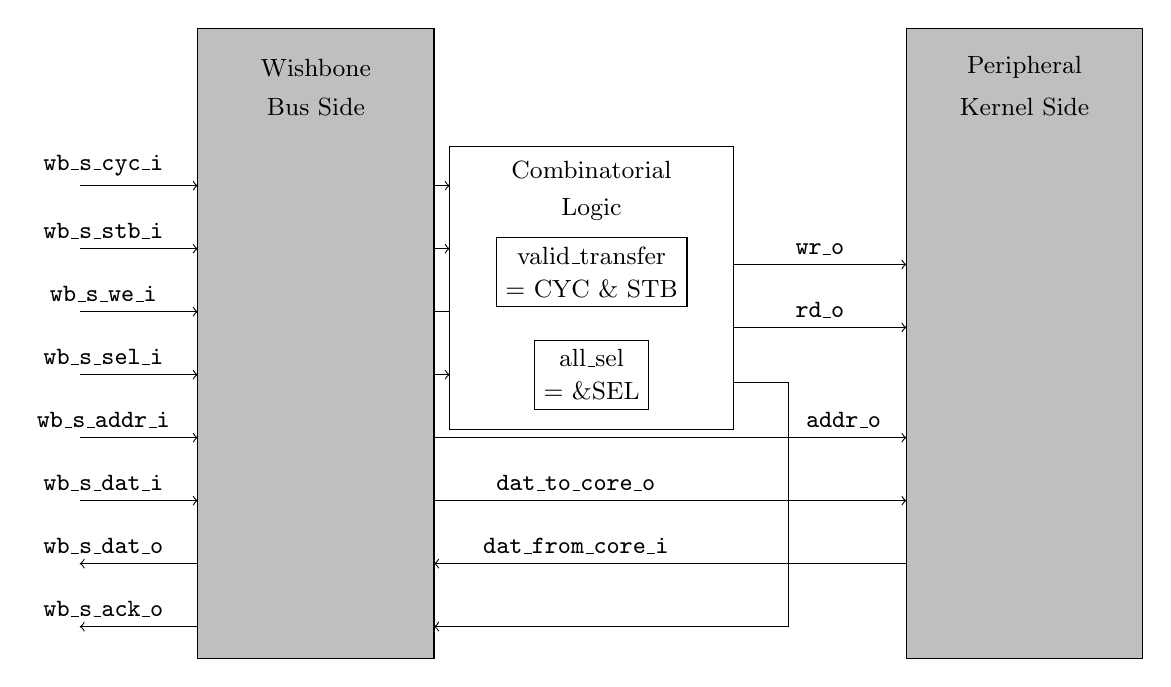
\begin{tikzpicture}
  % Bus-side box (left)
  \filldraw[fill=lightgray, draw=black] (0,0) rectangle (3,8);
  \node[align=center] at (1.5,7.5) {\small Wishbone};
  \node[align=center] at (1.5,7.0) {\small Bus Side};
  % Bus inputs
  \draw[->] (-1.5,6.0) -- (0,6.0) node[above,yshift=0.0cm,xshift=-1.2cm]{\small \texttt{wb\_s\_cyc\_i}};
  \draw[->] (-1.5,5.2) -- (0,5.2) node[above,yshift=0.0cm,xshift=-1.2cm]{\small \texttt{wb\_s\_stb\_i}};
  \draw[->] (-1.5,4.4) -- (0,4.4) node[above,yshift=0.0cm,xshift=-1.2cm]{\small \texttt{wb\_s\_we\_i}};
  \draw[->] (-1.5,3.6) -- (0,3.6) node[above,yshift=0.0cm,xshift=-1.2cm]{\small \texttt{wb\_s\_sel\_i}};
  \draw[->] (-1.5,2.8) -- (0,2.8) node[above,yshift=0.0cm,xshift=-1.2cm]{\small \texttt{wb\_s\_addr\_i}};
  \draw[->] (-1.5,2.0) -- (0,2.0) node[above,yshift=0.0cm,xshift=-1.2cm]{\small \texttt{wb\_s\_dat\_i}};
  \draw[<-] (-1.5,1.2) -- (0,1.2) node[above,yshift=0.0cm,xshift=-1.2cm]{\small \texttt{wb\_s\_dat\_o}};
  \draw[<-] (-1.5,0.4) -- (0,0.4) node[above,yshift=0.0cm,xshift=-1.2cm]{\small \texttt{wb\_s\_ack\_o}};
  % Logic box (centre)
  \filldraw[fill=white, draw=black] (3.2,2.9) rectangle (6.8,6.5);
  \node[align=center] at (5,6.2) {\small Combinatorial};
  \node[align=center] at (5,5.7) {\small Logic};
  % AND gate label
  \node[draw,align=center,fill=white] at (5,4.9) {\small valid\_transfer\\ \small = CYC \& STB};
  \node[draw,align=center,fill=white] at (5,3.6) {\small all\_sel\\ \small = \&SEL};
  % Connections bus→logic
  \draw[->] (3,6.0) -- (3.2,6);
  \draw[->] (3,5.2) -- (3.2,5.2);
  \draw[-]  (3,4.4) -- (3.2,4.4);
  \draw[->] (3,3.6) -- (3.2,3.6);
  % Kernel-side box (right)
  \filldraw[fill=lightgray, draw=black] (9,0) rectangle (12,8);
  \node[align=center] at (10.5,7.5) {\small Peripheral};
  \node[align=center] at (10.5,7.0) {\small Kernel Side};
  % addr passthrough
  \draw[->] (3,2.8) -- (9,2.8) node[midway,above, xshift=2.2cm]{\small \texttt{addr\_o}};
  % write data passthrough
  \draw[->] (3,2.0) -- (9,2.0) node[midway,above, xshift=-1.2cm]{\small \texttt{dat\_to\_core\_o}};
  % read data passthrough
  \draw[<-] (3,1.2) -- (9,1.2) node[midway,above, xshift=-1.2cm]{\small \texttt{dat\_from\_core\_i}};
  % wr_o from logic
  \draw[->] (6.8,5.0) -- (9,5.0) node[midway,above]{\small \texttt{wr\_o}};
  % rd_o from logic
  \draw[->] (6.8,4.2) -- (9,4.2) node[midway,above]{\small \texttt{rd\_o}};
  % ack_o back to bus
  \draw[->] (6.8,3.5) -- (7.5,3.5) -- (7.5,0.4) -- (3,0.4);
\end{tikzpicture}
\caption{as\_slave\_bpi -- Internal Signal Flow}
\label{fig:asSlaveBpi01}
\end{figure}

Table~\ref{tab:asSlaveBpiInt} lists the internal signals.

\begin{table}[H]
\caption{as\_slave\_bpi Internal Signals}
\label{tab:asSlaveBpiInt}
\centering
\begin{tabularx}{\textwidth}{|l |l |l |X|}
  \hline
  Signal & Type & Width & Description \\
  \hline
  \hline
  \texttt{valid\_transfer\_s} & logic & 1 & High when both CYC and STB are asserted.
    Indicates an active Wishbone bus cycle. \\
  \hline
  \texttt{all\_sel\_s}        & logic & 1 & High when all byte-select bits are set.
    Only full 64-bit word accesses are accepted. \\
  \hline
\end{tabularx}
\end{table}

\subsubsection{Instantiation}

The module is parameterised and instantiated as follows:

\begin{verbatim}
as_slave_bpi #(
    .addr_width ( 64 ),
    .data_width ( 64 )
) u_gpio_bpi (
    .rst_i              ( rst_i              ),
    .clk_i              ( clk_i              ),
    // kernel side
    .addr_o             ( addr_s             ),
    .dat_from_core_i    ( dat_from_core_s    ),
    .dat_to_core_o      ( dat_to_core_s      ),
    .wr_o               ( wr_s               ),
    .rd_o               ( rd_s               ),
    // wishbone side
    .wb_s_addr_i        ( wb_s_addr_i        ),
    .wb_s_dat_i         ( wb_s_dat_i         ),
    .wb_s_dat_o         ( wb_s_dat_o         ),
    .wb_s_we_i          ( wb_s_we_i          ),
    .wb_s_sel_i         ( wb_s_sel_i         ),
    .wb_s_stb_i         ( wb_s_stb_i         ),
    .wb_s_ack_o         ( wb_s_ack_o         ),
    .wb_s_cyc_i         ( wb_s_cyc_i         )
);
\end{verbatim}

\subsubsection{Limitations and Design Rules}

\begin{itemize}
  \item \textbf{Zero wait states only.}
    The peripheral kernel must provide read data combinatorially.
    If the kernel uses registered outputs, a wait-state mechanism
    (delayed ACK) must be added externally.
  \item \textbf{Full-word accesses only.}
    Sub-word byte or half-word accesses are not supported.
    The \texttt{SEL} check ensures that partial accesses are rejected silently.
  \item \textbf{No ERR\_O.}
    Bus errors are not signalled. Invalid accesses are simply not acknowledged
    (ACK stays low).
  \item \textbf{No burst support.}
    The module supports only Wishbone Classic single-cycle transfers.
    Pipeline or burst modes are not implemented.
  \item \textbf{Combinatorial ACK.}
    Connecting multiple slave BPIs in a shared-bus topology requires
    that ACK is only driven by the selected slave. Address decoding
    and ACK gating must be handled by the bus interconnect logic, not
    by this module.
\end{itemize}


